% ISPA revision, 2026-10-01. See 修订说明与证据核对.md before submission.
% Empirical values are archived DEVELOPMENT results, not newly performed runs.
% No synthetic numerical results are used in this document.
\documentclass[conference,compsoc]{IEEEtran}
\usepackage[T1]{fontenc}
\usepackage{amsmath,amssymb}
\interdisplaylinepenalty=2500
\usepackage{graphicx,booktabs,array,multirow}
\usepackage[nocompress]{cite}
\usepackage{xurl}
\usepackage{placeins}
\usepackage{tikz}
\usetikzlibrary{arrows.meta,positioning}
\graphicspath{{figures_revised/}}
\emergencystretch=1em
\newcommand{\clip}{\operatorname{clip}_{[0,1]}}
\newcommand{\med}{\operatorname{med}}
\newcommand{\mad}{\operatorname{MAD}}
\newcommand{\ind}{\mathbf{1}}
\newcommand{\norm}[1]{\left\lVert#1\right\rVert_2}
\newenvironment{compactitems}{\begin{itemize}\setlength{\itemsep}{1pt}}{\end{itemize}}
\begin{document}
\title{TTFL: Dual-Stream Trust Management for\ Robust Federated Learning at the Edge}
\author{\IEEEauthorblockN{Jiakai Zhou, Chao Bu, Shuo Zhang, Xinyu Liu}
\IEEEauthorblockA{School of Computer Science and Engineering\\
Tianjin University of Technology, Tianjin, China\\
Email: w1lsp0@stud.tjut.edu.cn, bc\_0722@163.com}}
\maketitle

\begin{abstract}
Federated learning must distinguish weak contributions caused by heterogeneous client data from updates that create a security risk. A single participation score can obscure this distinction: strict exclusion may suppress benign clients, whereas a favorable contribution history may delay restrictions on an attacker. We present TTFL, a server-assisted trust-management framework that retains historical utility and recent risk separately and translates them into recoverable restrictions and layer-specific aggregation. We specify the score ranges, temporal ordering, and aggregation boundary of a software prototype, and evaluate participation directly through admitted model tensors. An archived development study uses CIFAR-10, 20 clients, two seeds, and 30 communication rounds, with a disjoint 500-image server reference set. Without known-trigger probes, TTFL reduces mean benign client-round exclusion from 13.68\% to 4.30\% relative to a collapsed-state ablation under persistent backdoor injection, while final attack success rises from 5.34\% to 7.51\%. A known-trigger probe configuration lowers TTFL's final attack success to 2.72\% but raises benign exclusion to 17.98\%. These results identify a participation--security tradeoff rather than universal dominance. The evaluation is preliminary and does not establish hardware attestation security or generalization to unknown backdoors.
\end{abstract}

\begin{IEEEkeywords}
Federated learning, trust management, Non-IID data, backdoor attacks, client participation, edge computing
\end{IEEEkeywords}

\section{Introduction}
Federated learning (FL) coordinates local training without collecting all client training samples at a central server~\cite{mcmahan2017fedavg,kairouz2021flsurvey}. At the edge, differences in class coverage, sample counts, and device availability make client updates heterogeneous. An update that agrees poorly with a server reference may nevertheless contain useful information about an underrepresented population. Conversely, an attacker may contribute normally before injecting a targeted update~\cite{bagdasaryan2020backdoor}. Both cases require decisions about continued participation, beyond a one-round ranking of update quality.

Low utility may justify reduced weight or recoverable restriction, whereas sustained harmful behavior may justify stronger exclusion. A shared threshold can obscure this distinction. Separate state variables permit different persistence and recovery rules, although their observations need not be statistically independent.

Existing methods inspect update geometry~\cite{blanchard2017krum,yin2018byzantine}, agreement with a trusted reference~\cite{cao2021fltrust}, client histories~\cite{fung2020foolsgold,fldetector2022}, or model behavior and frequency structure~\cite{deepsight2022,flame2022,freqfed2024}. TTFL concentrates on the interface between such evidence and aggregation privileges. Historical utility retains a smoothed record of contribution quality. A separate risk stream retains warnings from server-side probes. Their values and the resulting restrictions determine which tensors of each update can contribute.

The contributions are an explicit dual-stream participation policy; its connection to layer gates and clipping, with an update-norm bound and risk-response calculation; and an analysis of matched development runs using accuracy, attack-window behavior, and benign-client exclusion. The results distinguish lowering attack success from removing an attacker and expose the cost of stronger probing.

The evaluated system is a Flower/PyTorch software prototype. Hardware-backed admission is a deployment extension, not an experimentally established component of this study. This separation makes the evidence boundary explicit: the measured comparisons concern update auditing and participation decisions.

\section{Related Work}
\textbf{Update aggregation and reference assistance.}
FedAvg weights local models by their training sample counts~\cite{mcmahan2017fedavg}. Krum uses distances between updates, and coordinate-wise trimmed aggregation reduces the influence of extreme coordinates~\cite{blanchard2017krum,yin2018byzantine}. These mechanisms address aggregation under adversarial inputs but do not by themselves define recoverable client participation. FLTrust uses a server-held root dataset to establish a reference update~\cite{cao2021fltrust}. Comparisons with reference-assisted methods must disclose both the source of these samples and whether the same reference is available to each method.

\textbf{Temporal and backdoor-oriented defenses.}
FoolsGold uses historical similarity to address Sybil behavior~\cite{fung2020foolsgold}; FLDetector predicts updates from historical information and identifies inconsistent clients~\cite{fldetector2022}. FLDetector therefore has client-removal behavior that can be evaluated directly; it should not be assigned an inapplicable detection metric merely because its state names differ from TTFL's. DeepSight inspects model-update characteristics~\cite{deepsight2022}. FLAME combines clustering, clipping, and noise~\cite{flame2022}, and FreqFed filters updates using frequency-domain structure~\cite{freqfed2024}. CrowdGuard uses collaborative backdoor detection~\cite{crowdguard2024}. These methods motivate stronger baselines, but the present numerical comparisons are limited to the implementations actually represented in the archived runs.

\textbf{Execution integrity.}
Trusted execution environments (TEEs) can protect selected execution and key-management components~\cite{r1_tee_integrity,xu2021distributed,r5_tee_mitigating}. Their guarantees depend on the protected code and data path. Authenticating an update-receiving agent does not establish the safety of external GPU training. The present evaluation makes no hardware trust-root claim.

\section{System Model and Evidence Boundary}
\subsection{Task, Server, and Adversary}
Let $W^{t-1}$ be the global model distributed in round $t$. Client $k$ returns an update $u_k^t=W_k^t-W^{t-1}$. An honest-but-curious server follows the stated algorithm and can inspect individual updates and audit statistics. Raw client training samples are not uploaded, but this restriction alone provides no formal privacy guarantee for updates or statistics. Cryptographic secure aggregation that hides individual updates is outside this auditing interface.

The usual sample-weighted objective is
\begin{equation}
 \min_W\sum_{k=1}^{K}p_k\mathcal L_k(W),\qquad
 p_k=\frac{|\mathcal D_k|}{\sum_j|\mathcal D_j|}.
\end{equation}
TTFL intentionally uses adaptive client-level trust weights rather than multiplying every survivor score by $p_k$. It consequently does not claim to implement an unbiased optimizer of this objective. This distinction matters for clients with different sample counts and for any claim about population utility.

The conceptual adversary can poison local examples or submit manipulated updates. The archived evaluation tests a narrower case: one designated client inserts a fixed trigger targeting class 0, either from round 1 or from round 11. The attack fraction is therefore $1/20=5\%$. This experiment does not validate six simultaneous attack types, a 30\% malicious population, or a 50\% Byzantine boundary. Client identities remain fixed within each run; adversarial re-registration and a general Sybil defense are not evaluated.

\subsection{Execution and Reference Assumptions}
The supplied client code includes a simulated TEE interface. In the development profile used here, client-reported telemetry does not determine trust decisions, and the runtime factor is set to $T_k^t=1$. No Kalman observation model, hardware quote latency, protected monitoring result, or GPU integrity guarantee is inferred from these simulations.

A deployment extension could protect an admission/signing agent while training remains outside the boundary. It would need an attested key and authenticated bindings among client identity, round, server challenge, global-model digest, and update digest. These are unvalidated extension requirements. Post-training manipulation remains in scope for that boundary; protected training would still permit poisoned inputs.

The evaluated server holds 500 labeled reference images selected from the CIFAR-10 training split, with 50 per class. These images are excluded from client training. The final 10,000-image test split is reserved for evaluation. All reference-assisted implementations use the same reference indices for a given comparison. TTFL remains reference-assisted even when a peer direction is available: behavioral probes still consume server-held samples. A peer fallback alone is not a data-free defense, and it does not solve trust bootstrapping in the first round.

\section{Dual-Stream Participation Policy}
Figure~\ref{fig:flow} shows the decision order. The method below describes the frozen development profile, with the numerical policy supplied as an in-memory reference artifact. Its historical update is an EMA of normalized utility; a decayed Beta model and a Kalman runtime filter are not part of the evaluated implementation.

\begin{figure}[t]
\centering
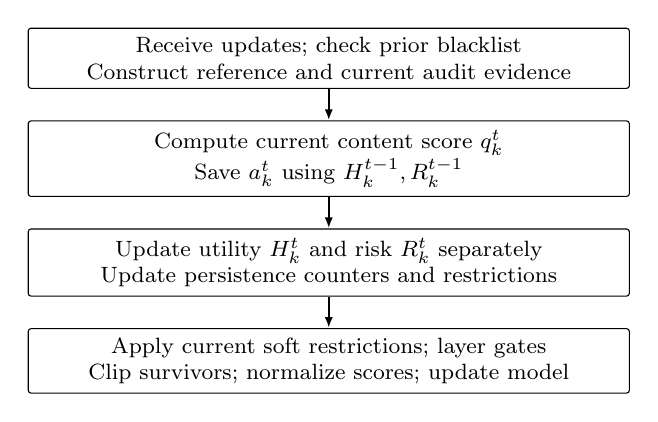
\begin{tikzpicture}[font=\footnotesize, node distance=4mm,
 b/.style={draw,rounded corners=1pt,align=center,text width=7.4cm,minimum height=7mm},
 a/.style={-{Latex[length=1.4mm]},thick}]
\node[b] (i) {Receive updates; check prior blacklist\\Construct reference and current audit evidence};
\node[b,below=of i] (s) {Compute current content score $q_k^t$\\Save $a_k^t$ using $H_k^{t-1},R_k^{t-1}$};
\node[b,below=of s] (h) {Update utility $H_k^t$ and risk $R_k^t$ separately\\Update persistence counters and restrictions};
\node[b,below=of h] (g) {Apply current soft restrictions; layer gates\\Clip survivors; normalize scores; update model};
\draw[a] (i)--(s);\draw[a] (s)--(h);\draw[a] (h)--(g);
\end{tikzpicture}
\caption{Decision order in the evaluated software. New blacklist decisions are checked on subsequent admission; current soft restrictions affect current aggregation. No hardware attestation is implied.}
\label{fig:flow}
\end{figure}

\subsection{Reference Direction and Current Utility}
The clean reference $g^t$ is a \emph{model update}, obtained by training a copy of $W^{t-1}$ for one pass over the server reference set using SGD (learning rate 0.01, momentum 0.9). Thus $g^t=W_{\rm ref}^t-W^{t-1}$ has the same descent convention as $u_k^t$; it is not the positive loss gradient. Vector comparisons exclude BatchNorm running statistics and counters. Norm denominators use a $10^{-9}$ stabilizer.

Define the soft similarity map $f(c)=\max(0,0.6+0.4c)$. For valid cosine values, $f(c)\in[0.2,1]$: an opposite direction retains a positive floor and is not automatically rejected. For at least two audited clients,
\begin{align}
 v_k^t &= f\bigl(\cos(u_k^t,g^t)\bigr),\\
 c_k^t &= \frac{\sum_{j\ne k}T_j^t f\bigl(\cos(u_k^t,u_j^t)\bigr)}{\sum_{j\ne k}T_j^t},\\
 q_k^t &= \clip\!\left(\frac{5c_k^t v_k^t}{4c_k^t+v_k^t+10^{-9}}\right).
\end{align}
The consistency score is zero if its denominator is zero; with only one client, the implementation uses $q_k^t=v_k^t$. The harmonic fusion gives greater emphasis to reference agreement. Peer agreement remains ambiguous under both collusion and legitimate heterogeneity.

\subsection{Historical Utility and Bounded Risk}
Let $\mu_t$ and $\sigma_t$ denote the mean and population standard deviation of current content scores. The implementation forms
\begin{align}
 z_k^t &= \frac{q_k^t-\mu_t}{\sigma_t+10^{-6}},\\
 \widetilde q_k^t &=0.4\frac{1}{1+\exp(-z_k^t)}
       +0.6\clip\!\left(\frac{q_k^t-0.4}{0.3}\right),\\
 H_k^t &=0.8H_k^{t-1}+0.2\widetilde q_k^t,\qquad H_k^0=0.5.
\end{align}
Relative performance and an absolute quality floor therefore both influence utility. History is updated on audited submissions. The studied runs have full participation; missing submissions are not zero-quality observations.

Each risk channel first maps its own statistic into $[0,1]$. A generic high-tail map is $\phi(x;b,s)=\clip((x-b)/s)$, with $s>0$. For example, the direction channel in the evaluated profile uses $\phi(\med_j\cos(u_j,g)-\cos(u_k,g);0,0.08)$. The activation-spectrum channel maps the dominant singular-value share $\xi_k$ as $\phi(\xi_k;0.15,0.08)$. The temporal channel uses the standard deviation of up to ten measured probe observations, mapping it with baseline 0.4 and scale 0.2 after at least five observations. These are heuristic calibration constants, not universal security thresholds.

The optional known-trigger channel evaluates right-bottom and left-top trigger templates. For each template, a target-class probability $x_k$ is compared with $b=\med_j x_j+2.5\max(\mad_j x_j,0.02)$ and scale $s=\max(0.05,0.8\max(\mad_j x_j,0.02))$. The larger normalized template score is retained. The remaining behavioral channel uses augmented-input predictive entropy and a round-dependent robust threshold; it is not an unbounded KL divergence or a trigger-independent proof of backdoor detection. The accompanying policy artifact records its history correction, sampling conditions, and constants.

Peer-tail evidence is smoothed separately with retention 0.7. Let $e_k^t$ be that value and $b_k^t$ the largest non-peer risk. The effective peer risk is
\begin{equation}
 \bar e_k^t=\begin{cases}
 0.6\min(e_k^t,b_k^t+0.12),&b_k^t<0.25,\\
 \min(e_k^t,b_k^t+0.12),&\text{otherwise}.
 \end{cases}
\end{equation}
The maximum of all bounded channels yields $r_k^t$. With initial risk $R_k^0=0.25$, the ordinary update is
\begin{equation}\label{eq:risk}
 R_k^t=0.85R_k^{t-1}+0.15r_k^t.
\end{equation}
An implemented override sets $R_k^t=1$ when the maximum risk is at least 0.99, at least two channels reach 0.90, and trigger risk reaches 0.52 or behavioral-probe risk reaches 0.98. This override changes the risk state; it does not retroactively recompute a previously saved aggregation score. A single low similarity value is therefore distinct from a current update restriction or a permanent ban.

\subsection{Restrictions, Counters, and Timing}
Before updating temporal states, the server saves
\begin{equation}\label{eq:score}
 a_k^t=(T_k^t)^3q_k^t\sqrt{H_k^{t-1}}(1-R_k^{t-1}).
\end{equation}
The current submission affects $q_k^t$ immediately. New utility and risk values then update restriction counters. Table~\ref{tab:states} distinguishes displayed states from actual aggregation controls. Counter time is the client's audited submissions; it is not elapsed wall-clock time. History-based isolation ends when the low-history streak resets. Risk isolation ends when both the soft-risk and accumulated-drift conditions cease to hold. Blacklisting is absorbing within a run.

\begin{table}[t]
\caption{State and eligibility rules in the frozen prototype. Full compound predicates are provided in the policy artifact.}
\label{tab:states}
\centering\footnotesize
\begin{tabular}{@{}>{\raggedright\arraybackslash}p{1.95cm}>{\raggedright\arraybackslash}p{6.05cm}@{}}
\toprule
Control & Condition and consequence\\
\midrule
Utility isolation & $H<0.26$ for five consecutive audited submissions. Exclude from aggregation while active; retain auditing. Low utility alone does not blacklist.\\
SUSPECT & Display when the soft-risk counter is positive or $R\ge0.59$ or peer risk $\ge0.59$, unless quarantined. This label alone does not imply zero weight.\\
QUARANTINE & Soft-risk counter $\ge5$ or drift-memory quarantine active. Exclude current aggregation; continue collecting recovery evidence.\\
Soft-risk count & Increase if $R>0.64$ and corroborating evidence is present; otherwise decrease by one, or two under the implemented relief condition.\\
BLACKLIST & Escalation priority: hard-risk count $\ge4$; trigger-combination count $\ge2$; corroborated drift count $\ge5$; or soft-risk count $\ge8$ with strong corroboration. Applied at subsequent admission.\\
NORMAL & No displayed suspicion/quarantine condition. A NORMAL label does not override utility isolation or layer rejection.\\
\bottomrule
\end{tabular}
\end{table}

Corroboration is essential to the policy. The hard-risk counter increases only if $R>0.90$, a probe/trigger or peer-plus-direction condition holds, and an earlier drift seed or a trigger warning is present. The trigger and drift routes use different persistent evidence. Their ordered Boolean predicates, threshold values, and decay rules are retained in the supplied numerical reference; neither a state name nor an EMA threshold alone fully specifies the implementation.

There is an implementation timing limitation: the candidate list is formed after current soft restrictions, but a new blacklist entry is not independently rechecked against every current candidate. Thus a newly blacklisted client is certainly rejected on its next submission; its current contribution depends on the soft and layer gates. Results below use observed tensor admission to measure blocking and do not equate a blacklist timestamp with immediate exclusion. Repairing that order would define a changed implementation requiring reevaluation.

\subsection{Layer Gates and Survivor Normalization}
Here a ``layer'' is an indexed state-dictionary tensor, including buffers, rather than an independently localized attacked semantic layer. Let $\mathcal A_t$ contain valid clients not excluded by the current aggregation controls. For tensor $l\in\{0,\ldots,L-1\}$, let $\bar u^{t,l}$ be the trust-weighted reference from those clients. The sensitivity components are
\begin{align}
 s_p^l&=\exp(-3l/L),\\
 s_u^l&=\frac{\norm{\bar u^{t,l}}}{\max_j\norm{\bar u^{t,j}}},\\
 s_s^l&=\clip\!\left(1-\frac{\sum_{k\in\mathcal A_t}T_k^t\cos(u_k^{t,l},\bar u^{t,l})}{\sum_{k\in\mathcal A_t}T_k^t}\right),\\
 s^l&=0.3s_p^l+0.4s_u^l+0.3s_s^l.
\end{align}
Zero reference norms use a unit denominator in the utility term; trust sums and cosine norms are stabilized. The depth term is a heuristic prior, not a quantified privacy guarantee. The utility term enters directly, as in the evaluated source, rather than through its complement. The threshold and clipping radius are
\begin{equation}
 \theta_l=0.05+0.15s^l,\qquad C_l=\frac{2}{s^l+0.01}.
\end{equation}
Consequently $\theta_l\in[0.05,0.20]$. These thresholds are on the same scale as $a_k^t\in[0,1]$ and replace the incompatible 0.4/1.2 parameterization. For example, $T=1,q=0.6,H=0.5,R=0.25$ gives $a\simeq0.318$ at startup; admission is possible but not guaranteed for other observations.

Define survivors $\Phi_l^t=\{k\in\mathcal A_t:a_k^t\ge\theta_l\}$. The implementation computes
\begin{align}
 w_k^{t,l}&=\frac{a_k^t}{\sum_{j\in\Phi_l^t}a_j^t+10^{-9}},\\
 \widehat u_k^{t,l}&=\frac{u_k^{t,l}}{\max(1,\norm{u_k^{t,l}}/C_l)},\\
 W^{t,l}&=W^{t-1,l}+\sum_{k\in\Phi_l^t}w_k^{t,l}\widehat u_k^{t,l}.
\end{align}
An empty survivor set gives a zero update. With the stabilizer, weights sum to slightly less than one, so this is survivor score normalization rather than an exact projection onto a simplex. All tensors share the same client score; their survivor sets are nested as thresholds increase. The mechanism varies filtering strictness across tensors and does not locate an attack independently for each client and layer.

\subsection{Round Algorithm and Analytical Properties}
The complete ordering is summarized below. The frozen numerical policy accompanies the manuscript so that the compound rules can be inspected without interpreting diagram arrows.
\begin{table}[t]
\caption{Round procedure for the evaluated TTFL profile.}
\label{tab:algorithm}
\centering\footnotesize
\begin{tabular}{@{}p{.3cm}p{7.7cm}@{}}
\toprule
1 & Distribute $W^{t-1}$; receive client models; reject identities already blacklisted. Form $u_k^t$ relative to the distributed model.\\
2 & Construct the clean reference on a model copy. Compute current content and scheduled behavioral evidence. Set $T_k^t=1$ in the software profile.\\
3 & Save scores $a_k^t$ using current content and prior $H,R$. Update utility, bounded risk, and the ordered compound restriction rules.\\
4 & Remove clients with current utility/risk isolation. Apply each layer threshold to the saved score; clip and normalize surviving contributions.\\
5 & Keep a tensor unchanged if no client survives. Save the global model and states; log admitted tensor counts and evaluation outcomes.\\
\bottomrule
\end{tabular}
\end{table}

For stationary, temporally uncorrelated utility inputs of variance $\sigma_q^2$, an EMA with retention $\rho_h$ has asymptotic variance
\begin{equation}
 \operatorname{Var}(H)=\frac{1-\rho_h}{1+\rho_h}\sigma_q^2.
\end{equation}
This explains smoothing under those assumptions; it is not an FL convergence proof or a detection guarantee. For a constant risk observation $r$ without the override, after $m$ audited submissions,
\begin{equation}
 R_{t+m}=r+(R_t-r)\rho_r^m.
\end{equation}
With $R_t=0.25$, $r=1$, and $\rho_r=0.85$, risk first exceeds 0.64 after five observations. Persistence conditions can add further delay. When observations return to zero, $R$ decays geometrically, but blacklist absorption and other counters can prevent eligibility from recovering. This is why a risk curve is insufficient evidence of participation recovery.

Finally, nonnegative normalized weights and clipping give
\begin{equation}
 \norm{W^{t,l}-W^{t-1,l}}
 \le \sum_{k\in\Phi_l^t}w_k^{t,l}\norm{\widehat u_k^{t,l}}
 \le C_l.
\end{equation}
The inequality applies to the floating-point aggregation before any buffer type conversion; it limits update magnitude, not harmful direction. For $K_t$ clients and $d$ compared coordinates, pairwise consistency costs $O(K_t^2d)$, while scoring and aggregation cost $O(K_td)$. Candidate-model probes add roughly $O(K_t m C_f)$ for $m$ evaluated inputs and forward cost $C_f$. These operations, rather than scalar state updates, dominate potential server scaling costs.

\section{Experimental Study}
\subsection{Protocol and Provenance}
The study uses archived protocol-v2 development runs: 24 standard runs, 12 runs with known-trigger probes, and eight attack-stop runs. Each condition uses seeds 20240925 and 20240926. Tables are recomputed from per-run records, using the final round for both accuracy and ASR and sample standard deviations across the two seeds. These are development observations, not independent final validation or statistical-significance tests. The original remote console logs are not all present in the local archive; numerical consistency checks do not substitute for a fresh training replication.

The task is CIFAR-10 with a ResNet-18~\cite{he2016resnet}: the first convolution is $3\times3$ with stride 1, max pooling is removed, and the classifier has ten outputs. The development profile initializes randomly. It partitions 49,500 training images across 20 clients, after reserving 500 images for the server. Clients 0--9 receive IID partitions, 10--14 use Dirichlet concentration 1.0, and 15--19 use concentration 0.1. Client partitions have no shared training pool. Partition and initialization records support matched comparisons; seeds change initialization, client splits, and stochastic training, while the balanced proxy-selection rule is fixed.

Training uses 30 rounds, full participation, one local epoch per round, batch size 32, and SGD with learning rate 0.001 and momentum 0.9. The local optimizer is recreated each round; there is no learning-rate schedule or nonzero weight decay in this profile. Augmentation uses random cropping and horizontal flipping. The server reference pass uses batch size 64. BatchNorm buffers are exchanged and aggregated as state-dictionary tensors, although similarity computations exclude their running statistics and counters. The manifests identify five visible GPUs; no validated end-to-end deployment timing is inferred from that allocation.

The persistent and delayed attacks use client 1, target class 0, a bottom-right $3\times3$ trigger, and a local poisoning rate of 1.0. The delayed client trains benignly through round 10. No-attack runs use the same triggered evaluation to measure the background target-hit rate. Target-class examples are excluded, leaving 9,000 eligible CIFAR-10 test examples. Untargeted attacks are not assigned an ASR, and separate semantic or clean-label performance is not inferred from this trigger test.

\subsection{Comparators and Metrics}
FedAvg and a local FLTrust implementation provide aggregation comparisons. The collapsed-state ablation uses the same utility and risk observations as TTFL but combines them as $D_k=\clip(H_k(1-R_k))$. It weights with $q_k\sqrt{D_k^{t-1}}$ and excludes when the current $D_k<0.26$. This collapses the \emph{decision state}, retaining both estimators and additional blacklist rules. No threshold sweep matches benign exclusion, so the comparison does not establish an optimal frontier.

For an attack transform $\mathcal T_a$ and target $y_a$, we use
\begin{equation}
 \mathrm{ASR}_a^t=
 \frac{\sum_{(x,y)\in\mathcal E:y\ne y_a}
 \ind[\arg\max f_{W^t}(\mathcal T_a(x))=y_a]}
 {|\{(x,y)\in\mathcal E:y\ne y_a\}|}.
\end{equation}
Attack-window mean and peak ASR measure transient harm. The no-attack target-hit rate on the same transformed examples is the relevant background comparison; a nominal ten-class chance level is not a backdoor-removal criterion.

Let $I_{k,t}$ be the number of tensors that admit client $k$, and $\mathcal B$ the configured benign identities. Mean complete exclusion is
\begin{equation}
 E_{\rm benign}=\frac{\sum_{t=1}^{30}\sum_{k\in\mathcal B}\ind[I_{k,t}=0]}{30|\mathcal B|}.
\end{equation}
The ever-excluded rate counts distinct benign identities excluded at least once. Neither metric is a permanent-ban FPR. Permanent-ban FPR would use the final blacklist and its actual benign-client denominator; unsupported percentages under that definition are not retained. Missing audit rows are never interpreted as zero contribution without explicit archived exclusion evidence. N/A for a comparator means the necessary participation audit is unavailable, not that it excluded no clients.

\subsection{Utility and Security Without Known-Trigger Probes}
Table~\ref{tab:main} and Fig.~\ref{fig:results} show the standard profile, denoted K0: known-trigger probes are disabled and heavy probes use a rotation modulus of five, with priority checks for suspicious clients. Without attacks, TTFL yields $57.34\pm0.33\%$ accuracy and $5.33\pm0.94\%$ mean benign exclusion. The collapsed-state ablation yields $57.12\pm0.91\%$ accuracy but $14.75\pm2.24\%$ exclusion. Thus similar global accuracy can coexist with materially different access to aggregation.

\begin{table*}[t]
\caption{Standard development profile K0: mean $\pm$ sample standard deviation over two seeds. All metrics are percentages. Final metrics use round 30. ``Benign excl.'' counts completely excluded client-rounds; ``ever excl.'' counts distinct benign clients. No-attack ASR entries are background target-hit rates.}
\label{tab:main}
\centering\footnotesize
\setlength{\tabcolsep}{4pt}
\begin{tabular*}{\textwidth}{@{\extracolsep{\fill}}llccccc@{}}
\toprule
Scenario & Method & Accuracy & Final ASR & Window ASR & Benign excl. & Ever excl.\\
\midrule
% BEGIN GENERATED STANDARD TABLE
No attack & FedAvg & $56.53\pm0.38$ & $4.28\pm0.68$ & -- & -- & -- \\
No attack & FLTrust & $54.60\pm1.62$ & $5.40\pm3.57$ & -- & -- & -- \\
No attack & Single-state & $57.12\pm0.91$ & $4.71\pm1.08$ & -- & $14.75\pm2.24$ & $30.00\pm0.00$ \\
No attack & TTFL & $57.34\pm0.33$ & $4.32\pm0.71$ & -- & $5.33\pm0.94$ & $10.00\pm0.00$ \\
\midrule
Persistent & FedAvg & $54.61\pm0.95$ & $9.51\pm1.42$ & $18.67\pm0.92$ & -- & -- \\
Persistent & FLTrust & $48.03\pm6.87$ & $18.12\pm24.54$ & $19.11\pm1.16$ & -- & -- \\
Persistent & Single-state & $56.03\pm0.10$ & $5.34\pm3.64$ & $13.81\pm2.15$ & $13.68\pm2.98$ & $28.95\pm3.72$ \\
Persistent & TTFL & $56.08\pm0.57$ & $7.51\pm1.72$ & $15.04\pm1.54$ & $4.30\pm0.62$ & $7.89\pm3.72$ \\
\midrule
Delayed & FedAvg & $55.27\pm0.77$ & $9.38\pm1.16$ & $13.76\pm1.84$ & -- & -- \\
Delayed & FLTrust & $48.80\pm5.56$ & $17.08\pm23.33$ & $18.30\pm1.39$ & -- & -- \\
Delayed & Single-state & $55.85\pm0.77$ & $10.73\pm2.02$ & $10.49\pm1.72$ & $16.14\pm1.98$ & $31.58\pm0.00$ \\
Delayed & TTFL & $56.68\pm0.50$ & $6.25\pm2.57$ & $11.55\pm1.88$ & $5.79\pm1.98$ & $15.79\pm0.00$ \\
% END GENERATED STANDARD TABLE
\bottomrule
\end{tabular*}
\end{table*}

\begin{figure*}[t]
\centering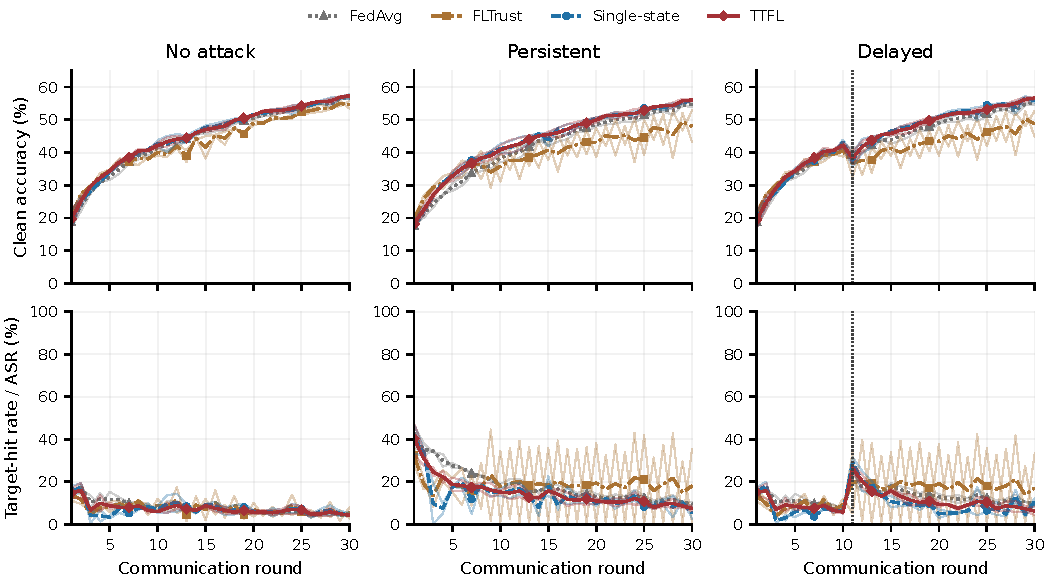
\includegraphics[width=\textwidth]{fig_results.pdf}
\caption{K0 development trajectories. Thick curves show two-seed means; faint curves show the individual seeds, not confidence intervals. The bottom-left panel is the target-hit rate without poisoning. The dotted vertical line in the delayed condition marks attack onset at round 11.}
\label{fig:results}
\end{figure*}

Under persistent injection, TTFL retains more benign participation: mean exclusion falls from $13.68\%$ to $4.30\%$, a 9.38-point difference at the displayed precision. However, final ASR increases from $5.34\%$ to $7.51\%$, and attack-window ASR increases from $13.81\%$ to $15.04\%$. The two methods therefore trade attack suppression against benign participation in this setting. The data do not support describing the dual stream as uniformly more accurate or more secure.

Under delayed injection, TTFL's final ASR is $6.25\pm2.57\%$, compared with $10.73\pm2.02\%$ for the collapsed state. Mean benign exclusion is $5.79\%$ versus $16.14\%$. Yet TTFL's attack-window ASR remains slightly higher, $11.55\%$ versus $10.49\%$. A favorable final checkpoint can conceal earlier attack exposure. In both attacked K0 scenarios, the archived audit records do not show complete exclusion of the attacker within 30 rounds. Reduced ASR must therefore not be presented as proof of client removal.

FLTrust exhibits substantial seed variation in these runs, including $18.12\pm24.54\%$ final ASR under persistent injection. With only two seeds, this observation calls for additional controlled runs and implementation checks rather than a general ranking of defenses. FLAME, FLDetector, and FreqFed remain relevant comparison targets, but their previously listed summary values lack a matching run archive and are not treated as measured results here.

\subsection{Probe Dependence and Actual Participation}
The K1 profile enables known-trigger probes and performs heavy probing each round. Initial models, partitions, and training code are matched to K0 in the archived paired comparison. Two probe settings change together, so the difference cannot be attributed solely to trigger knowledge or solely to scheduling.

Figure~\ref{fig:probe} shows the resulting tradeoff. For persistent injection, TTFL final ASR changes from $7.51\%$ to $2.72\%$, and attack-window ASR from $15.04\%$ to $5.58\%$. Benign exclusion increases from $4.30\%$ to $17.98\%$. Under delayed injection, final ASR changes from $6.25\%$ to $2.57\%$ while benign exclusion rises from $5.79\%$ to $15.70\%$. K1 also raises TTFL benign exclusion without attacks to $15.50\%$. Stronger evidence can therefore improve attack suppression while imposing a participation cost on legitimate clients.

\begin{figure*}[t]
\centering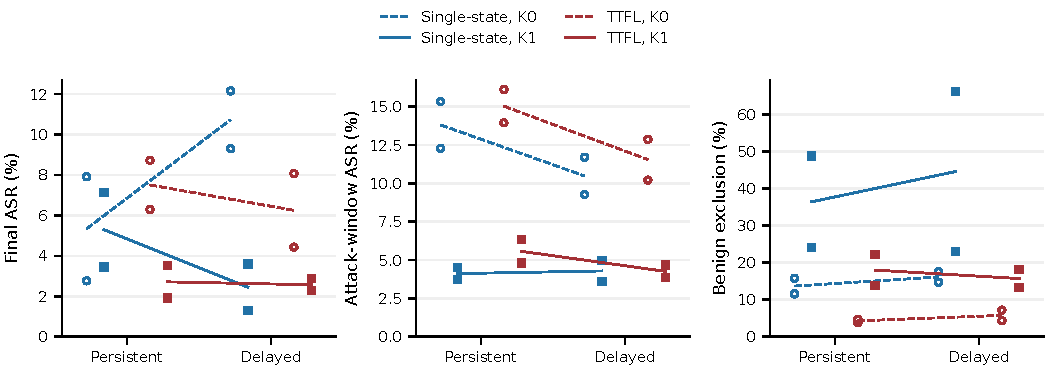
\includegraphics[width=\textwidth]{fig_probe_tradeoff.pdf}
\caption{Probe-configuration dependence. Open circles/dashed lines denote K0; filled squares/solid lines denote K1. Points show individual seeds; lines connect scenario means. K1 combines known triggers with more frequent heavy probing. The right panel exposes the accompanying benign-participation cost.}
\label{fig:probe}
\end{figure*}

\begin{figure*}[t]
\centering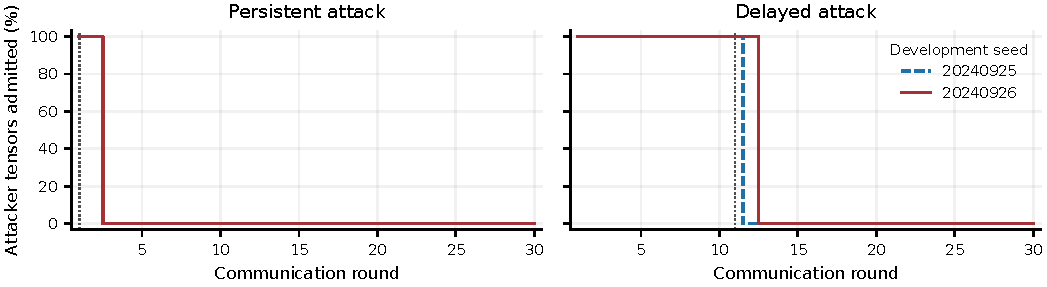
\includegraphics[width=\textwidth]{fig_attacker_participation.pdf}
\caption{Actual attacker tensor admission for TTFL under K1. The two curves are separate seeds. This is an admission-count fraction, not aggregation weight. First complete exclusion occurs in round 3 for persistent injection and rounds 12/13 for delayed injection. Vertical dotted lines mark attack onset.}
\label{fig:participation}
\end{figure*}

Figure~\ref{fig:participation} measures blocking directly. With K1, TTFL first completely excludes the persistent attacker in round 3 for both seeds, two rounds after attack onset. In the delayed case the first exclusion occurs in rounds 12 and 13, one and two rounds after onset. These are aggregation-blocking delays, not first-detection times. A collapsed-state run excludes the client before delayed injection starts; that event cannot be credited as detection of the later attack. Normal-client contribution weights and local tail accuracy are not reconstructed from tensor counts.

\subsection{Attack-Stop Study and Recovery Limits}
Eight additional K0 runs activate the attacker in rounds 3--9 and stop poisoning at round 10. For TTFL, the attacker is never completely excluded during that attack window in either seed. Consequently these runs provide no measured transition from attack-induced complete exclusion back to participation, and a recovery delay is not reported as zero. One collapsed-state run remains excluded through round 30; the other is not excluded during the attack window. A decrease in post-stop ASR describes model behavior and is not evidence of client recovery. A benign-client distribution-shift experiment with a documented restriction and return to nontrivial weight is still needed to establish that benefit.

\FloatBarrier
\section{Discussion and Limitations}
The results identify a conditional tradeoff: separate states preserve more benign participation, while known-trigger probing improves attack suppression at a participation cost. Both configurations assume a clean server reference; reference-size, class-bias, and fully reference-free variants remain unevaluated.

Two development seeds, one dataset/model, and one attacker identity do not establish broad robustness. Held-out seeds, matched-exclusion threshold sweeps, modern defense implementations, partial participation, adaptive attacks, and multi-attack benchmarks remain necessary. Fixed identities leave reputation-reset attacks unresolved.

Implementation behavior must be distinguished from the intended policy. Saved scores use prior risk, compound counters add delay, and a new blacklist entry is enforced at the next admission check. Missing or nonfinite evidence requires an explicit fail-closed interface; the current archive does not validate such malformed-input handling. Per-candidate model restoration, BatchNorm-buffer behavior, and processing-order invariance require dedicated checks before claiming reproducible security decisions. The numerical reference does not establish these end-to-end properties.

No measured end-to-end TDX latency, attestation throughput, or protected GPU training result is available for this profile. Earlier component summaries cannot be transferred to the changed experiment. Pairwise consistency and model probes suggest substantial server cost, but a client-count sweep and isolated phase timings are required to quantify scalability. The present evidence supports a study of participation control in a server-assisted FL prototype, not an edge-deployment performance guarantee.

\section{Conclusion}
TTFL separates historical contribution from recent security risk and connects both to recoverable restrictions and layer-specific aggregation. The explicit score ranges and decision order clarify what is controlled immediately and what depends on accumulated evidence. In the two-seed development study, TTFL reduces benign exclusion relative to a collapsed-state decision rule, with attack suppression depending strongly on the probe configuration. Reporting attack-window ASR and actual admission reveals limitations that final accuracy and permanent-ban counts alone conceal. Further validation should test the participation--security tradeoff with held-out seeds, matched thresholds, biased or smaller reference sets, and measured system costs.

\section*{Acknowledgments}
OpenAI ChatGPT/Codex assisted with manuscript restructuring, language editing, and preparation of evidence-extraction and plotting scripts. Experimental values were taken from existing archived records; no generated sample values are reported as measurements.

\bibliographystyle{Template/IEEEtran}
\bibliography{ispa2026_references_revised}
\end{document}
